% Options for packages loaded elsewhere
\PassOptionsToPackage{unicode}{hyperref}
\PassOptionsToPackage{hyphens}{url}
%
\documentclass[
]{report}
\usepackage{lmodern}
\usepackage{amssymb,amsmath}
\usepackage{ifxetex,ifluatex}
\ifnum 0\ifxetex 1\fi\ifluatex 1\fi=0 % if pdftex
  \usepackage[T1]{fontenc}
  \usepackage[utf8]{inputenc}
  \usepackage{textcomp} % provide euro and other symbols
\else % if luatex or xetex
  \usepackage{unicode-math}
  \defaultfontfeatures{Scale=MatchLowercase}
  \defaultfontfeatures[\rmfamily]{Ligatures=TeX,Scale=1}
\fi
% Use upquote if available, for straight quotes in verbatim environments
\IfFileExists{upquote.sty}{\usepackage{upquote}}{}
\IfFileExists{microtype.sty}{% use microtype if available
  \usepackage[]{microtype}
  \UseMicrotypeSet[protrusion]{basicmath} % disable protrusion for tt fonts
}{}
\makeatletter
\@ifundefined{KOMAClassName}{% if non-KOMA class
  \IfFileExists{parskip.sty}{%
    \usepackage{parskip}
  }{% else
    \setlength{\parindent}{0pt}
    \setlength{\parskip}{6pt plus 2pt minus 1pt}}
}{% if KOMA class
  \KOMAoptions{parskip=half}}
\makeatother
\usepackage{xcolor}
\IfFileExists{xurl.sty}{\usepackage{xurl}}{} % add URL line breaks if available
\IfFileExists{bookmark.sty}{\usepackage{bookmark}}{\usepackage{hyperref}}
\hypersetup{
  pdftitle={  STAT 216 Activity Coursepack},
  hidelinks,
  pdfcreator={LaTeX via pandoc}}
\urlstyle{same} % disable monospaced font for URLs
\usepackage{longtable,booktabs}
% Correct order of tables after \paragraph or \subparagraph
\usepackage{etoolbox}
\makeatletter
\patchcmd\longtable{\par}{\if@noskipsec\mbox{}\fi\par}{}{}
\makeatother
% Allow footnotes in longtable head/foot
\IfFileExists{footnotehyper.sty}{\usepackage{footnotehyper}}{\usepackage{footnote}}
\makesavenoteenv{longtable}
\usepackage{graphicx,grffile}
\makeatletter
\def\maxwidth{\ifdim\Gin@nat@width>\linewidth\linewidth\else\Gin@nat@width\fi}
\def\maxheight{\ifdim\Gin@nat@height>\textheight\textheight\else\Gin@nat@height\fi}
\makeatother
% Scale images if necessary, so that they will not overflow the page
% margins by default, and it is still possible to overwrite the defaults
% using explicit options in \includegraphics[width, height, ...]{}
\setkeys{Gin}{width=\maxwidth,height=\maxheight,keepaspectratio}
% Set default figure placement to htbp
\makeatletter
\def\fps@figure{htbp}
\makeatother
\setlength{\emergencystretch}{3em} % prevent overfull lines
\providecommand{\tightlist}{%
  \setlength{\itemsep}{0pt}\setlength{\parskip}{0pt}}
\setcounter{secnumdepth}{5}
\usepackage{booktabs}
\usepackage{geometry}
\usepackage[none]{hyphenat}
\usepackage{titlesec}
\usepackage{longtable}


\pagestyle{plain}

%%%% Set margins?... doesn't work
\setlength{\topmargin}{-1cm}
\addtolength{\evensidemargin}{-1cm}
\addtolength{\oddsidemargin}{-1cm}
\addtolength{\textheight}{1.8cm}
\addtolength{\textwidth}{2cm}

\renewcommand*{\chaptername}{Activity}

\titleformat{\chapter}[display]
{\bfseries\Large}
{\filleft\MakeUppercase{\chaptertitlename} \Huge\thechapter}
{3ex}
{\titlerule
\vspace{1.5ex}%
\filright}
[\vspace{1.5ex}%
\titlerule]
\titlespacing*{\chapter}{0pt}{-40pt}{20pt}
\usepackage[]{natbib}
\bibliographystyle{plainnat}

\title{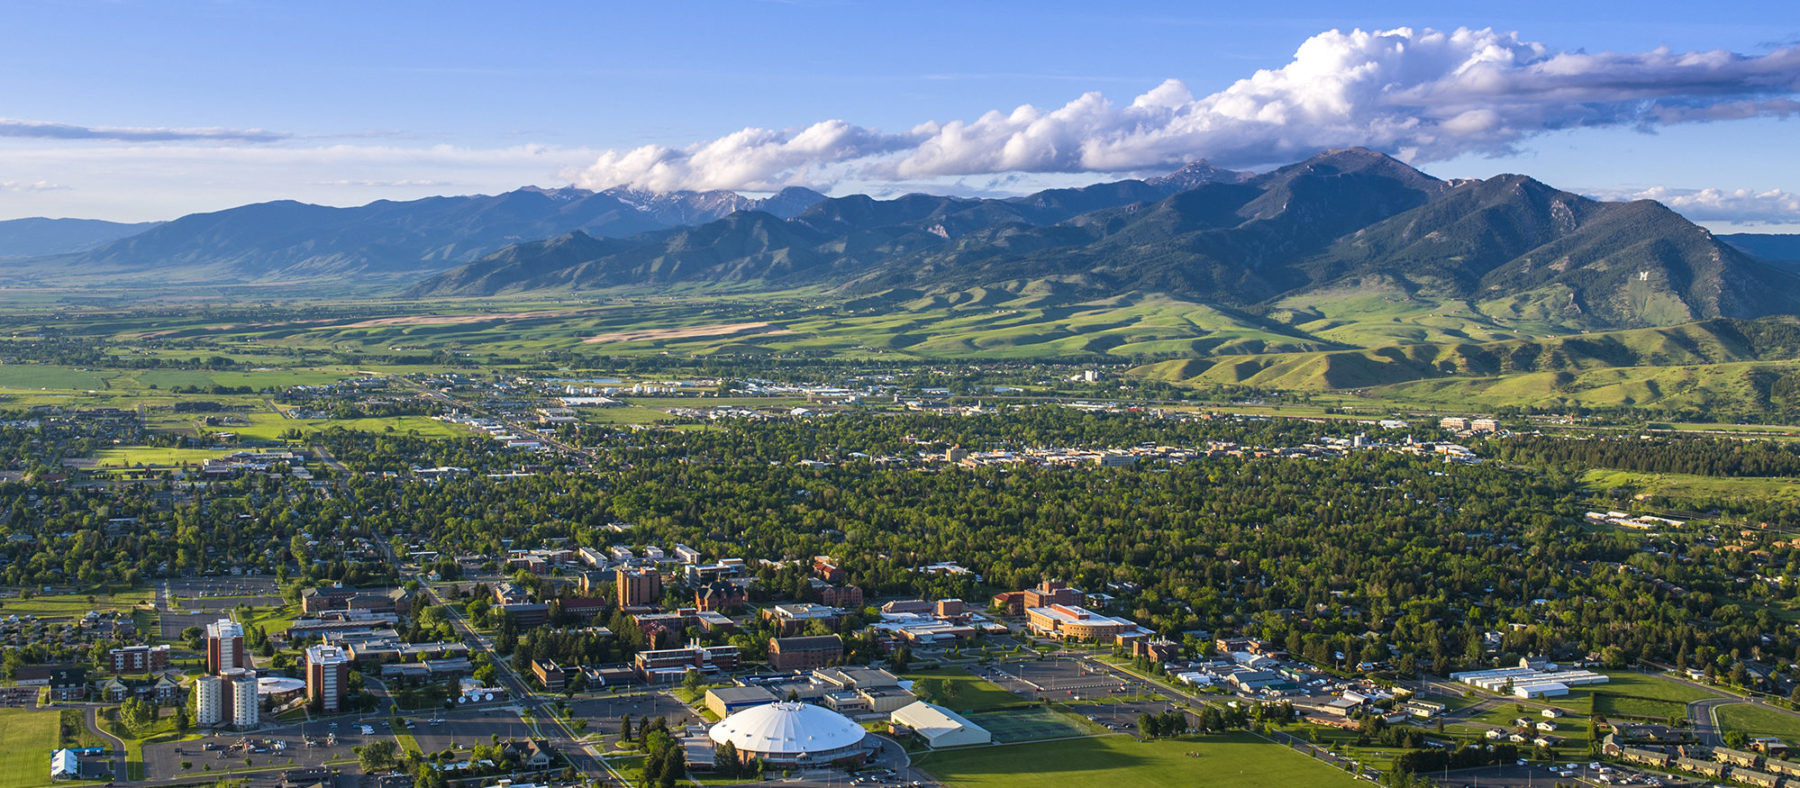
\includegraphics[width=5in,height=\textheight]{images/msu-campus.jpg}
\vspace{1cm}\\
STAT 216 Activity Coursepack}
\usepackage{etoolbox}
\makeatletter
\providecommand{\subtitle}[1]{% add subtitle to \maketitle
  \apptocmd{\@title}{\par {\large #1 \par}}{}{}
}
\makeatother
\subtitle{Fall 2020}
\author{}
\date{\vspace{-2.5em}}

\begin{document}
\maketitle

{
\setcounter{tocdepth}{0}
\tableofcontents
}
\hypertarget{preface}{%
\chapter*{Preface}\label{preface}}
\addcontentsline{toc}{chapter}{Preface}

This coursepack accompanies the textbook for STAT 216: Introduction to Statistics at Montana State University. Each of the activities in this workbook is designed to target specific learning outcomes of the course, giving you practice with important statistical concepts in a group setting with instructor guidance. Bring this workbook with you to class each week, and take notes in the workbook as you would your own notes. A well-written complete workbook will provide an optimal study guide for exams!

\hypertarget{fall-2020-calendar-of-in-class-activities}{%
\chapter*{Fall 2020 Calendar of In-Class Activities}\label{fall-2020-calendar-of-in-class-activities}}
\addcontentsline{toc}{chapter}{Fall 2020 Calendar of In-Class Activities}

Placeholder

\hypertarget{martian-alphabet}{%
\chapter{Martian Alphabet}\label{martian-alphabet}}

Placeholder

\hypertarget{learning-outcomes}{%
\section{Learning outcomes}\label{learning-outcomes}}

\hypertarget{terminology-review}{%
\section{Terminology review}\label{terminology-review}}

\hypertarget{can-you-read-martian}{%
\section{Can you read ``Martian''?}\label{can-you-read-martian}}

\hypertarget{steps-of-the-statistical-investigation-process}{%
\subsection{Steps of the statistical investigation process}\label{steps-of-the-statistical-investigation-process}}

\hypertarget{take-home-messages}{%
\section{Take home messages}\label{take-home-messages}}

\hypertarget{additional-notes}{%
\section{Additional notes}\label{additional-notes}}

\hypertarget{study-design}{%
\chapter{Study Design}\label{study-design}}

Placeholder

\hypertarget{learning-outcomes}{%
\section{Learning outcomes}\label{learning-outcomes}}

\hypertarget{terminology-review}{%
\section{Terminology review}\label{terminology-review}}

\hypertarget{types-of-sampling-bias}{%
\section{Types of sampling bias}\label{types-of-sampling-bias}}

\hypertarget{study-design-1}{%
\section{Study design}\label{study-design-1}}

\hypertarget{additional-notes}{%
\section{Additional notes}\label{additional-notes}}

\hypertarget{current-population-survey}{%
\chapter{Current Population Survey}\label{current-population-survey}}

Placeholder

\hypertarget{learning-outcomes}{%
\section{Learning outcomes}\label{learning-outcomes}}

\hypertarget{terminology-review}{%
\section{Terminology review}\label{terminology-review}}

\hypertarget{current-population-survey-1985}{%
\section{``Current'' Population Survey: 1985}\label{current-population-survey-1985}}

\hypertarget{vocabulary-review}{%
\subsection{Vocabulary review}\label{vocabulary-review}}

\hypertarget{r-code}{%
\subsection{\texorpdfstring{\texttt{R} code}{R code}}\label{r-code}}

\hypertarget{displaying-a-single-categorical-variable}{%
\subsection{Displaying a single categorical variable}\label{displaying-a-single-categorical-variable}}

\hypertarget{displaying-two-categorical-variables}{%
\subsection{Displaying two categorical variables}\label{displaying-two-categorical-variables}}

\hypertarget{probability}{%
\section{Probability}\label{probability}}

\hypertarget{additional-notes}{%
\section{Additional notes}\label{additional-notes}}

\hypertarget{imdb-movie-reviews}{%
\chapter{IMDb Movie Reviews}\label{imdb-movie-reviews}}

Placeholder

\hypertarget{learning-objectives}{%
\section{Learning objectives}\label{learning-objectives}}

\hypertarget{terminology-review}{%
\section{Terminology review}\label{terminology-review}}

\hypertarget{movies-released-in-2016}{%
\section{Movies released in 2016}\label{movies-released-in-2016}}

\hypertarget{vocabulary-review}{%
\section{Vocabulary review}\label{vocabulary-review}}

\hypertarget{summarizing-a-single-quantitative-variable}{%
\section{Summarizing a single quantitative variable}\label{summarizing-a-single-quantitative-variable}}

\hypertarget{displaying-a-single-quantitative-variable}{%
\section{Displaying a single quantitative variable}\label{displaying-a-single-quantitative-variable}}

\hypertarget{displaying-a-single-categorical-and-single-quantitative-variable}{%
\section{Displaying a single categorical and single quantitative variable}\label{displaying-a-single-categorical-and-single-quantitative-variable}}

\hypertarget{additional-notes}{%
\section{Additional notes}\label{additional-notes}}

\hypertarget{movie-profits}{%
\chapter{Movie Profits}\label{movie-profits}}

Placeholder

\hypertarget{learning-objectives}{%
\section{Learning objectives}\label{learning-objectives}}

\hypertarget{terminology-review}{%
\section{Terminology review}\label{terminology-review}}

\hypertarget{movies-released-in-2016}{%
\section{Movies released in 2016}\label{movies-released-in-2016}}

\hypertarget{vocabulary-review}{%
\subsection{Vocabulary review}\label{vocabulary-review}}

\hypertarget{correlation}{%
\subsection{Correlation}\label{correlation}}

\hypertarget{slope}{%
\subsection{Slope}\label{slope}}

\hypertarget{residuals}{%
\subsection{Residuals}\label{residuals}}

\hypertarget{coefficient-of-determination-r-squared}{%
\subsection{Coefficient of determination (R-squared)}\label{coefficient-of-determination-r-squared}}

\hypertarget{multivariate-plots}{%
\subsection{Multivariate plots}\label{multivariate-plots}}

\hypertarget{additional-notes}{%
\section{Additional notes}\label{additional-notes}}

\hypertarget{handedness-of-male-boxers}{%
\chapter{Handedness of Male Boxers}\label{handedness-of-male-boxers}}

Placeholder

\hypertarget{learning-objectives}{%
\section{Learning objectives}\label{learning-objectives}}

\hypertarget{terminology-review}{%
\section{Terminology review}\label{terminology-review}}

\hypertarget{steps-of-the-statistical-investigation-process}{%
\section{Steps of the statistical investigation process}\label{steps-of-the-statistical-investigation-process}}

\hypertarget{handedness-of-male-boxers-1}{%
\section{Handedness of male boxers}\label{handedness-of-male-boxers-1}}

\hypertarget{summary-statistics-review}{%
\subsection{Summary statistics review}\label{summary-statistics-review}}

\hypertarget{ask-a-research-question}{%
\subsection{Ask a research question}\label{ask-a-research-question}}

\hypertarget{design-a-study-and-collect-data}{%
\subsection{Design a study and collect data}\label{design-a-study-and-collect-data}}

\hypertarget{summarize-and-visualize-the-data}{%
\subsection{Summarize and visualize the data}\label{summarize-and-visualize-the-data}}

\hypertarget{use-statistical-analysis-methods-to-draw-inferences-from-the-data}{%
\subsection{Use statistical analysis methods to draw inferences from the data}\label{use-statistical-analysis-methods-to-draw-inferences-from-the-data}}

\hypertarget{communicate-the-results-and-answer-the-research-question}{%
\subsection{Communicate the results and answer the research question}\label{communicate-the-results-and-answer-the-research-question}}

\hypertarget{revisit-and-look-forward}{%
\subsection{Revisit and look forward}\label{revisit-and-look-forward}}

\hypertarget{additional-notes}{%
\section{Additional notes}\label{additional-notes}}

\hypertarget{winter-sports-helmet-use-and-head-injuries}{%
\chapter{Winter Sports Helmet Use and Head Injuries}\label{winter-sports-helmet-use-and-head-injuries}}

Placeholder

\hypertarget{learning-objectives}{%
\section{Learning objectives}\label{learning-objectives}}

\hypertarget{terminology-review}{%
\section{Terminology review}\label{terminology-review}}

\hypertarget{helmet-use-and-head-injuries}{%
\section{Helmet Use and Head Injuries}\label{helmet-use-and-head-injuries}}

\hypertarget{vocabulary-review}{%
\subsection{Vocabulary review}\label{vocabulary-review}}

\hypertarget{ask-a-research-question}{%
\subsection{Ask a research question}\label{ask-a-research-question}}

\hypertarget{summarize-and-visualize-the-data}{%
\subsection{Summarize and visualize the data}\label{summarize-and-visualize-the-data}}

\hypertarget{use-statistical-analysis-methods-to-draw-inferences-from-the-data}{%
\subsection{Use statistical analysis methods to draw inferences from the data}\label{use-statistical-analysis-methods-to-draw-inferences-from-the-data}}

\hypertarget{types-of-errors}{%
\subsection{Types of errors}\label{types-of-errors}}

\hypertarget{additional-notes}{%
\section{Additional notes}\label{additional-notes}}

\hypertarget{covid-19-and-air-pollution}{%
\chapter{COVID-19 and Air Pollution}\label{covid-19-and-air-pollution}}

Placeholder

\hypertarget{learning-outcomes}{%
\section{Learning outcomes}\label{learning-outcomes}}

\hypertarget{terminology-review}{%
\section{Terminology review}\label{terminology-review}}

\hypertarget{covid-19-and-air-pollution-1}{%
\section{COVID-19 and air pollution}\label{covid-19-and-air-pollution-1}}

\hypertarget{vocabulary-review}{%
\subsection{Vocabulary review}\label{vocabulary-review}}

\hypertarget{ask-a-research-question}{%
\subsection{Ask a research question}\label{ask-a-research-question}}

\hypertarget{summarize-and-visualize-the-data}{%
\subsection{Summarize and visualize the data}\label{summarize-and-visualize-the-data}}

\hypertarget{use-statistical-inferential-methods-to-draw-inferences-from-the-data}{%
\subsection{Use statistical inferential methods to draw inferences from the data}\label{use-statistical-inferential-methods-to-draw-inferences-from-the-data}}

\hypertarget{communicate-the-results-and-answer-the-research-question.}{%
\subsection{Communicate the results and answer the research question.}\label{communicate-the-results-and-answer-the-research-question.}}

\hypertarget{revisit-and-look-forward}{%
\subsection{Revisit and look forward}\label{revisit-and-look-forward}}

\hypertarget{additional-notes}{%
\section{Additional notes}\label{additional-notes}}

\hypertarget{weather-patterns-and-record-snowfall}{%
\chapter{Weather Patterns and Record Snowfall}\label{weather-patterns-and-record-snowfall}}

Placeholder

\hypertarget{learning-objectives}{%
\section{Learning objectives}\label{learning-objectives}}

\hypertarget{terminology-review}{%
\section{Terminology review}\label{terminology-review}}

\hypertarget{weather-patterns-and-record-snowfall-1}{%
\section{Weather Patterns and Record snowfall}\label{weather-patterns-and-record-snowfall-1}}

\hypertarget{quantitative-variables-review}{%
\subsection{Quantitative variables review}\label{quantitative-variables-review}}

\hypertarget{ask-a-research-question.}{%
\subsection{Ask a research question.}\label{ask-a-research-question.}}

\hypertarget{summarize-and-visualize-the-data}{%
\subsection{Summarize and visualize the data}\label{summarize-and-visualize-the-data}}

\hypertarget{use-statistical-inferential-methods-to-draw-inferences-from-the-data}{%
\subsection{Use statistical inferential methods to draw inferences from the data}\label{use-statistical-inferential-methods-to-draw-inferences-from-the-data}}

\hypertarget{communicate-the-results-and-answer-the-research-question}{%
\subsection{Communicate the results and answer the research question}\label{communicate-the-results-and-answer-the-research-question}}

\hypertarget{revisit-and-look-rorward}{%
\subsection{Revisit and look rorward}\label{revisit-and-look-rorward}}

\hypertarget{additional-notes}{%
\section{Additional notes}\label{additional-notes}}

\hypertarget{hand-dexterity}{%
\chapter{Hand Dexterity}\label{hand-dexterity}}

Placeholder

\hypertarget{learning-outcomes}{%
\section{Learning outcomes}\label{learning-outcomes}}

\hypertarget{terminology-review}{%
\section{Terminology review}\label{terminology-review}}

\hypertarget{hand-dexterity-1}{%
\section{Hand dexterity}\label{hand-dexterity-1}}

\hypertarget{vocabulary-review}{%
\subsection{Vocabulary review}\label{vocabulary-review}}

\hypertarget{conditions-for-the-least-squares-line}{%
\subsection{Conditions for the least squares line}\label{conditions-for-the-least-squares-line}}

\hypertarget{ask-a-research-question}{%
\subsection{Ask a research question}\label{ask-a-research-question}}

\hypertarget{summarize-and-visualize-the-data}{%
\subsection{Summarize and visualize the data}\label{summarize-and-visualize-the-data}}

\hypertarget{use-statistical-inferential-methods-to-draw-inferences-from-the-data}{%
\subsection{Use statistical inferential methods to draw inferences from the data}\label{use-statistical-inferential-methods-to-draw-inferences-from-the-data}}

\hypertarget{communicate-the-results-and-answer-the-research-question}{%
\subsection{Communicate the results and answer the research question}\label{communicate-the-results-and-answer-the-research-question}}

\hypertarget{revisit-and-look-forward}{%
\subsection{Revisit and look forward}\label{revisit-and-look-forward}}

\hypertarget{additional-notes}{%
\section{Additional notes}\label{additional-notes}}

\end{document}
